% !TeX root = ../0_Manuscript.tex

\section{Enhanced BBI platform model and simulation \ddc}
\label{chap:2_goodPractices;sect:enhancedBBIPlatforms}
In this section, I propose platform enhancements over the state-of-the-art \bbi platform previously introduced.
These improvements aim at being low-cost, fast, and easy to set up, to represent an interesting addition without drastically increasing the platform financial cost.
Eventually, I am able to draw conclusions on such improvements thanks to simulation results.

    \subsection{Matching the generator output impedance \ddcu}
    \label{chap:2_goodPractices;sect:enhancedBBIPlatforms;subsect:bbiGenImpMatch}
    % !TeX root = ../0_Manuscript.tex

\begin{figure}[H]
    \centering
    \begin{subfigure}{0.45\textwidth}
        \includegraphics[width=1.0\textwidth, center]{2_goodPractices/figures/model2ProbeManuscrit.pdf}
        \caption{Enhanced \bbi platform model. It describes the generator, the \bbi probe, the transmission line, the IC (1 k\textomega\xspace resistor), the default platform grounding (both 150 \textOmega\xspace resistors), and the enhancements highlighted in red, which are: creating an approximate impedance matching for the generator, and bypassing the poor grounding with low impedance copper wires.}
        \label{fig:bbiPracticeImpGnd}
    \end{subfigure}
    \hspace{0.045\textwidth}
    \begin{subfigure}{0.45\textwidth}
        \includegraphics[width=1.0\textwidth, center]{2_goodPractices/figures/SIMPLE_BBI_2.pdf}
        \caption{Simulation results of the enhanced \bbi model. \textcolor{RoyalBlue}{Blue}: ideal voltage pulse (-140 V, 10 ns). \textcolor{OliveGreen}{Green}: effective signal applied on the IC backside. \textcolor{orange}{Orange}: generator output. \textcolor{Purple}{Purple}: IC ground current. The dotted waveforms are those observed in Fig. \ref{fig:bbiPracticeBadGndSignals}. The most obvious observed improvements concern the set points, which are fully respected, in addition to the drastic ringing reduction, leading to better temporal control.}
        \label{fig:bbiPracticeImpGndSignals}
    \end{subfigure}
    \caption{\bbi platform enhanced electrical model developed for my thesis to quickly evaluate various platform parameters, alongside the model simulation results.}
    \label{fig:bbiImpGndGlobalFig}
\end{figure}

    The first proposed improvement concerns the generated voltage pulse characteristics.
    As I have shown previously, the various set point parameters are not met.
    In a fault injection context, it is an undesirable behavior, as it is required to finely control the generated pulse to produce controlled disturbances into the targeted IC.
    Therefore, and because most high-speed high voltage pulse generators are specified to be loaded with a precise impedance, I simply propose to connect a known load directly at the output of the generator.
    In my model, a \fiftyOhms{50} resistor is loaded at the generator output, as illustrated in red in Fig. \ref{fig:bbiPracticeImpGnd}.
    Thus, the generator sees the impedance network formed by the compensation load, the IC, the transmission line, and the grounding installation.
    However, because the grounding installation is platform-dependent, it is required, to perform a better impedance matching of the generator output, to improve the grounding, which leads to the other platform enhancement described in the following section.

    \subsection{Improving the grounding installation \ddcu}
    \label{chap:2_goodPractices;sect:enhancedBBIPlatforms;subsect:bbiGndBetter}
    In many platforms, the grounding installation might be perfectly fine, and the following section may not apply to them.
    However, with my platform, I quickly observed that the grounding impedance was far from negligible.
    Indeed, with an average IC impedance around 1 k\textOmega\xspace, and inter-equipment ground impedance around 150 \textOmega\xspace, it represents a 15 \% increase in the total impedance seen by the generator.
    Therefore, to transfer a maximum amount of energy into the IC, especially in areas where the IC impedance might be closer to the grounding impedance, it is required to cancel as much as possible the latter.

    To that end, I propose a simple setup modification.
    It consists in keeping the platform as is, and adding short copper wires between equipment grounds.
    Therefore, they shunt the platform's ground and creates a low-impedance path for electric charges, thus allowing the previous section approximate impedance matching to perform better.

    \subsection{Simulation results \ddcu}
    \label{chap:2_goodPractices;sect:enhancedBBIPlatforms;subsect:simRes}
    To verify the soundness of the previously proposed enhancements, I performed simulations thanks to the model presented in Fig. \ref{fig:bbiPracticeImpGnd}. The simulation results are shown in Fig. \ref{fig:bbiPracticeImpGndSignals}.

    In that case, unlike in the state-of-the-art platform, the voltage set point is almost met concerning the received pulse (green waveform), with a slight undershoot of 6\%.
    It is mirrored on the IC ground current waveform, where the ringing is drastically reduced, which leads to a steeper and more accurate pulse.
    It is especially noticeable when directly comparing the state-of-the-art waveforms in dotted lines.
    Concerning the generator pulse (orange waveform), it is still distorted as the ringing has not disappeared, but is less of a concern since the waveform of interest is the one effectively applied to the IC backside.
        \subsubsection{Load dependency \ddcno}
        \label{chap:2_goodPractices;sect:enhancedBBIPlatforms;subsect:simRes;subsubsect:loadDep}
        To further analyze the benefits of the proposed improvements, I performed, as for the state-of-the-art platform, additional simulations with various loads.
        As before, 250 \textOmega\xspace and 2 k\textOmega\xspace were chosen to have a common point of comparison.
        As I stated previously, these values are chosen to match the average typical value of my IC target when thinned down to 50 µ, up to 700 µm.
        
\begin{figure}[ht]
    \centering
    \begin{subfigure}{0.48\textwidth}
        \centering
        \includegraphics[width=1.0\textwidth, center]{2_goodPractices/figures/SIMPLE_BBI_2_0_IC250.pdf}
        \caption{Enhanced \bbi platform simulation results with an IC load equals to 250 \textOmega\xspace.}
        \label{fig:bbiPracticeImpGndICLoad0}
    \end{subfigure}
    \hfill
    \begin{subfigure}{0.48\textwidth}
        \centering
        \includegraphics[width=1.0\textwidth, center]{2_goodPractices/figures/SIMPLE_BBI_2_0_IC2k.pdf}
        \caption{Enhanced \bbi platform simulation results with an IC load equals to 2 k\textOmega\xspace.}
        \label{fig:bbiPracticeImpGndICLoad1}
    \end{subfigure}
    \caption{Enhanced \bbi platform simulation results with different IC load values.}
    \label{fig:bbiImpGndIcLoadVar}
\end{figure}

        Fig. \ref{fig:bbiImpGndIcLoadVar} presents the simulation results for such loads.
        For both loads, the measured voltage moves away from the set point by around 7 \% in each case.
        It represents a 14 \% range around the -140 V set point, which is immensely better than in the previous platform.
        It is still not perfect, but the platform is overall less dependent on the IC load, which is desirable to have a repeatable voltage pulse across the entire IC backside.

        Then, quite naturally, for the 250 \textOmega\xspace load, the current is higher than for the 1 k\textOmega\xspace, and with the 2 k\textOmega\xspace, it is lower.
        In addition to that, thanks to the 50 \textOmega\xspace resistor placed at the generator output, it reduces the range in which the effective load (the compensation load in parallel with the IC) changes.
        Indeed, it goes from around 42 \textOmega\xspace to about 49 \textOmega\xspace, instead of going from 250 \textOmega\xspace to 2 k\textOmega\xspace in the previous case.
        Eventually, in addition to all of the above, these enhancements have also drastically reduced ringing, which contributes to the applied pulse amplitude being closer to the set point.

    \subsection{Simulation conclusions \ddcno}
    All of this leads to better control over the various platform parameters, allowing for more accurate and shorter pulses, closer to the expectations.
    In addition to that, the platform is less design dependent thanks to the minimization of impedance mismatch and poor grounding installation.
    It leads to a better time accuracy, enabling potentially more controllable fault injections.
%         the 250 \textOmega\xspace load
%        Concerning the 250 \textOmega\xspace load results, displayed in Fig. \ref{fig:bbiPracticeImpGndICLoad0}.

\section{Actual enhanced BBI platform \ddcpu}
The previous models being a useful tool to draw quick conclusions and predictions, it does not represent the reality.
To that end, I set up the various presented enhancements in an actual \bbi platform to verify the soundness of all the outcomes.
In the first place, I am going to discuss how to perform the approximate impedance matching.
Then, I will explain how to set up an efficient grounding bypass.
Thereafter, I will take a look at actual measurements, allowing to spot the improvements.

    \subsection{Generator impedance matching in practice \ddcu}
%    \textcolor{orange}{Add pictures of real platform impedance matching.}
    % !TeX root = ../0_Manuscript.tex

%\begin{figure}[ht]
%    \centering
%    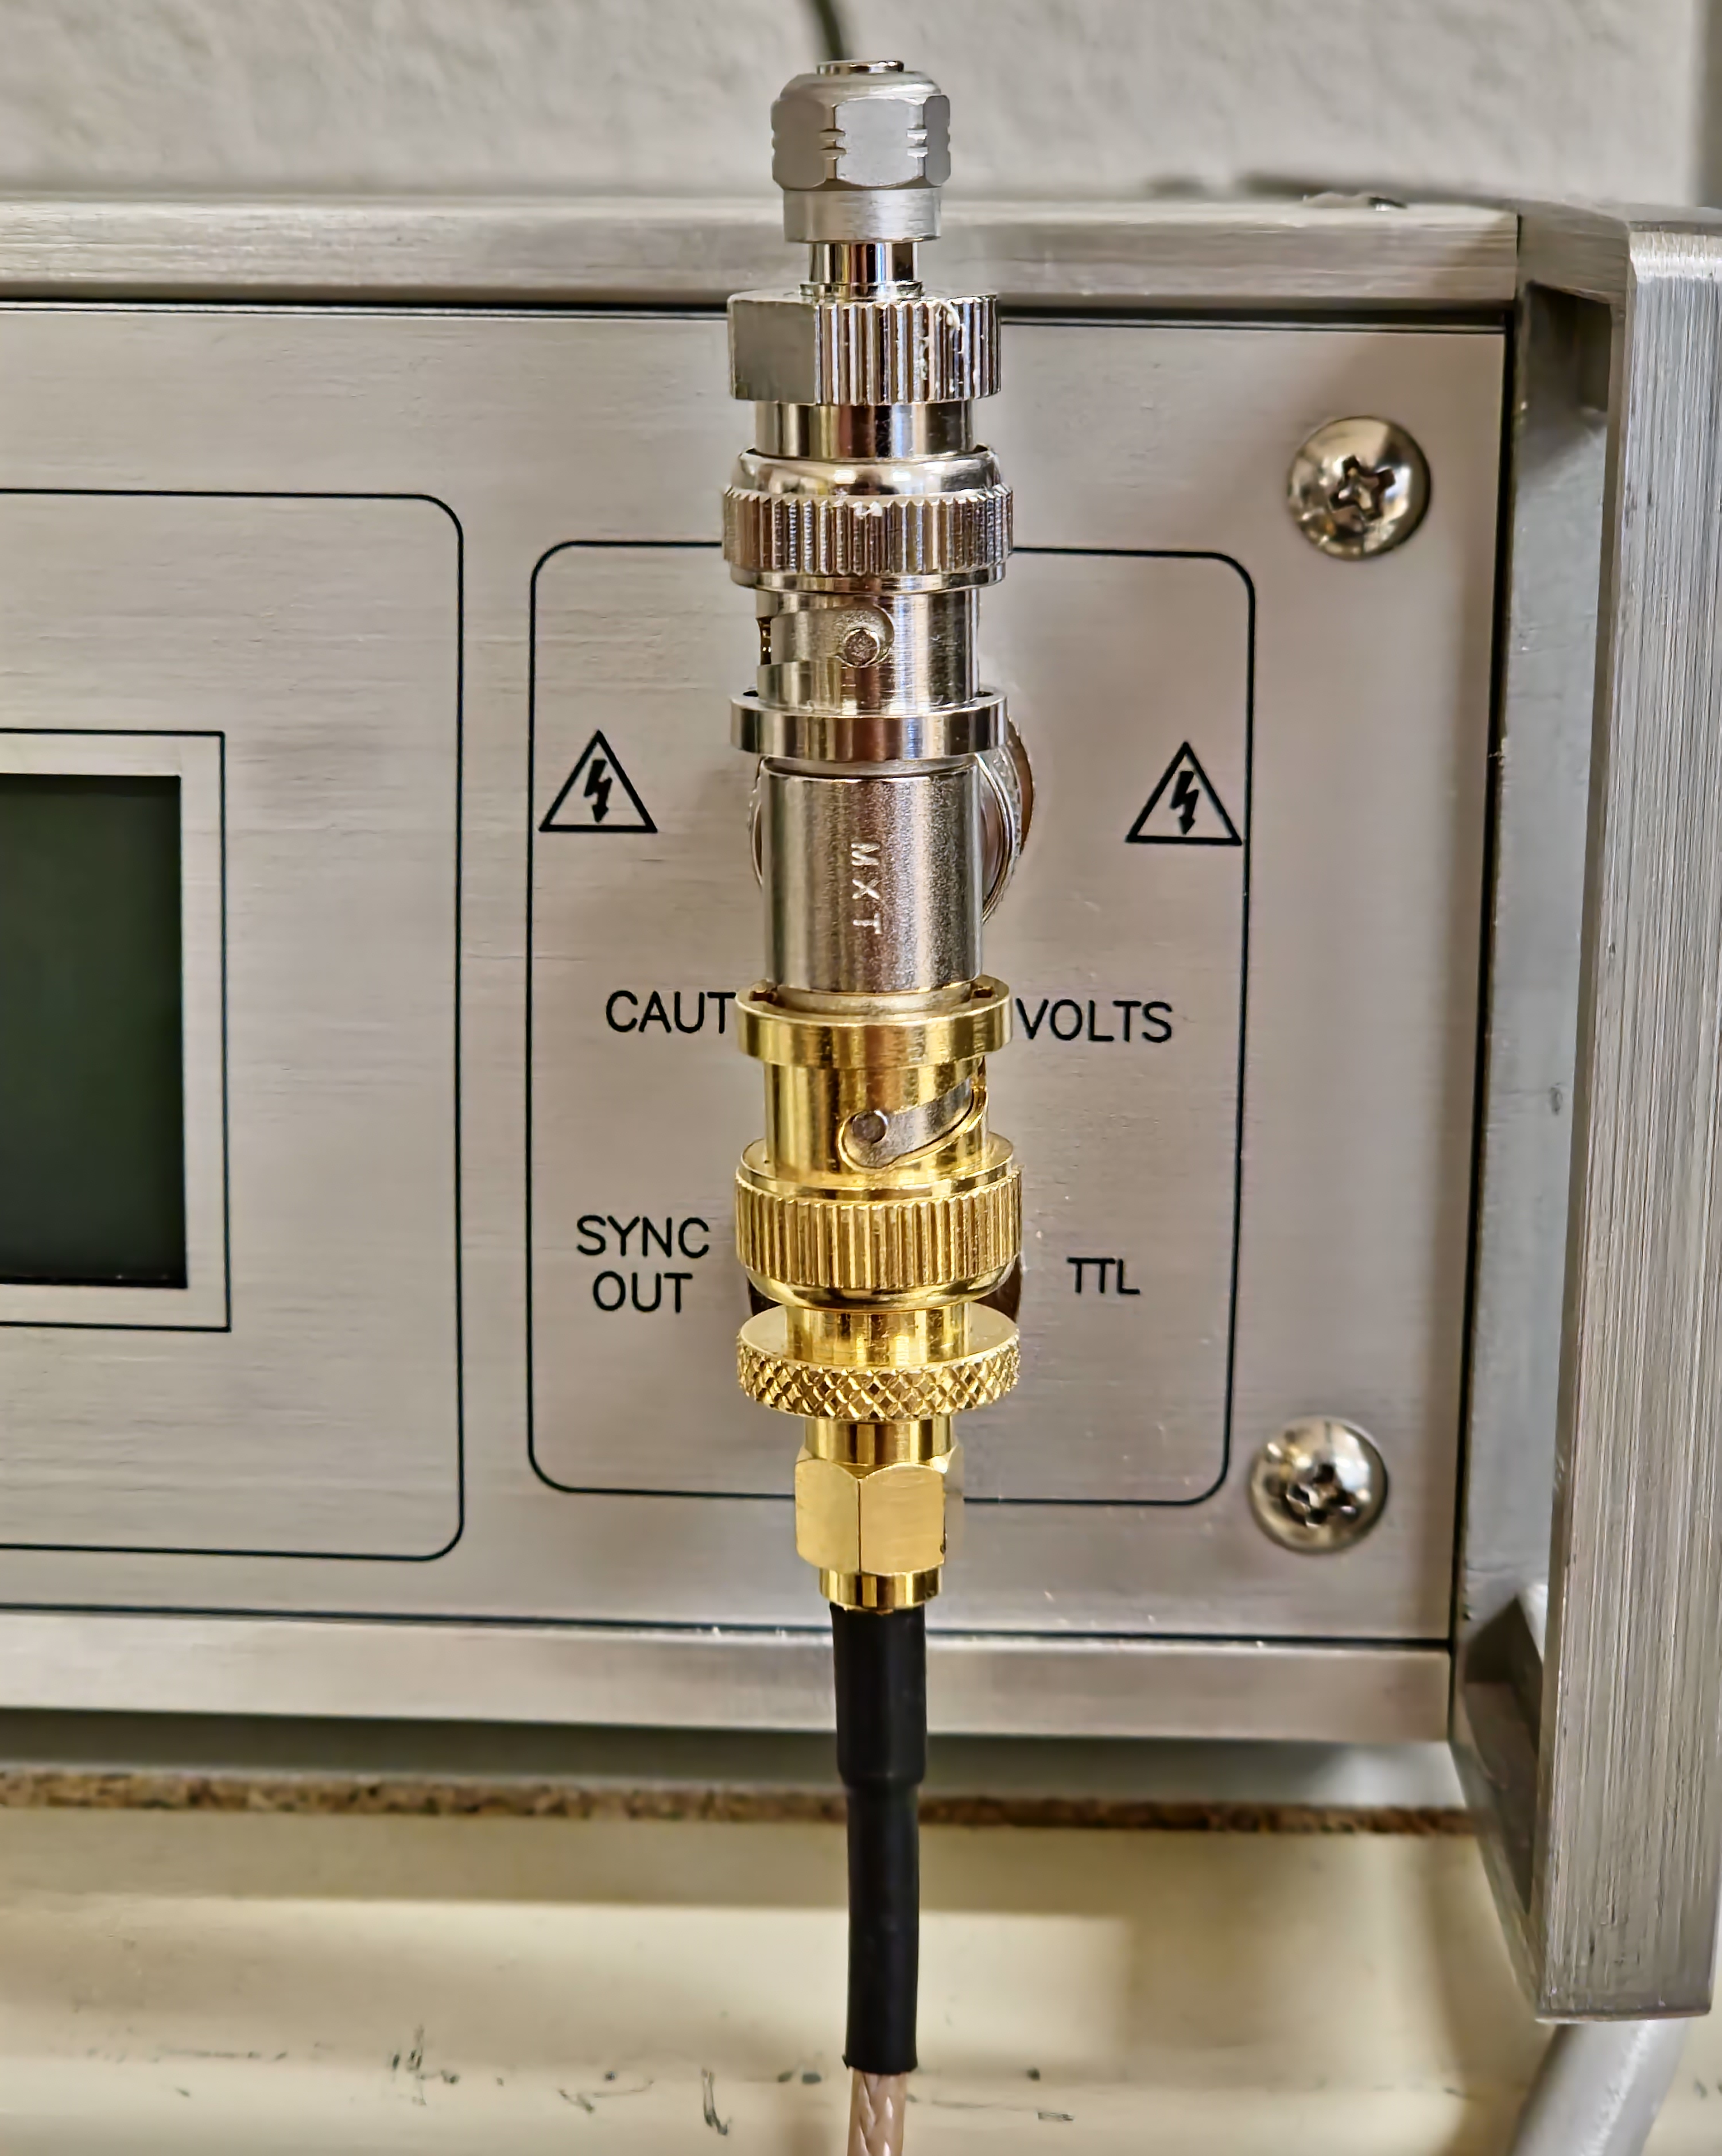
\includegraphics[width=0.3\textwidth, center]{2_goodPractices/figures/impMatchPicture.png}
%    \caption{Actual implementation of the proposed impedance matching.}
%    \label{fig:impMatchPhoto}
%\end{figure}


\begin{figure}[ht]
    \centering
%    \hfill
    \begin{subfigure}{0.48\textwidth}
        \centering
        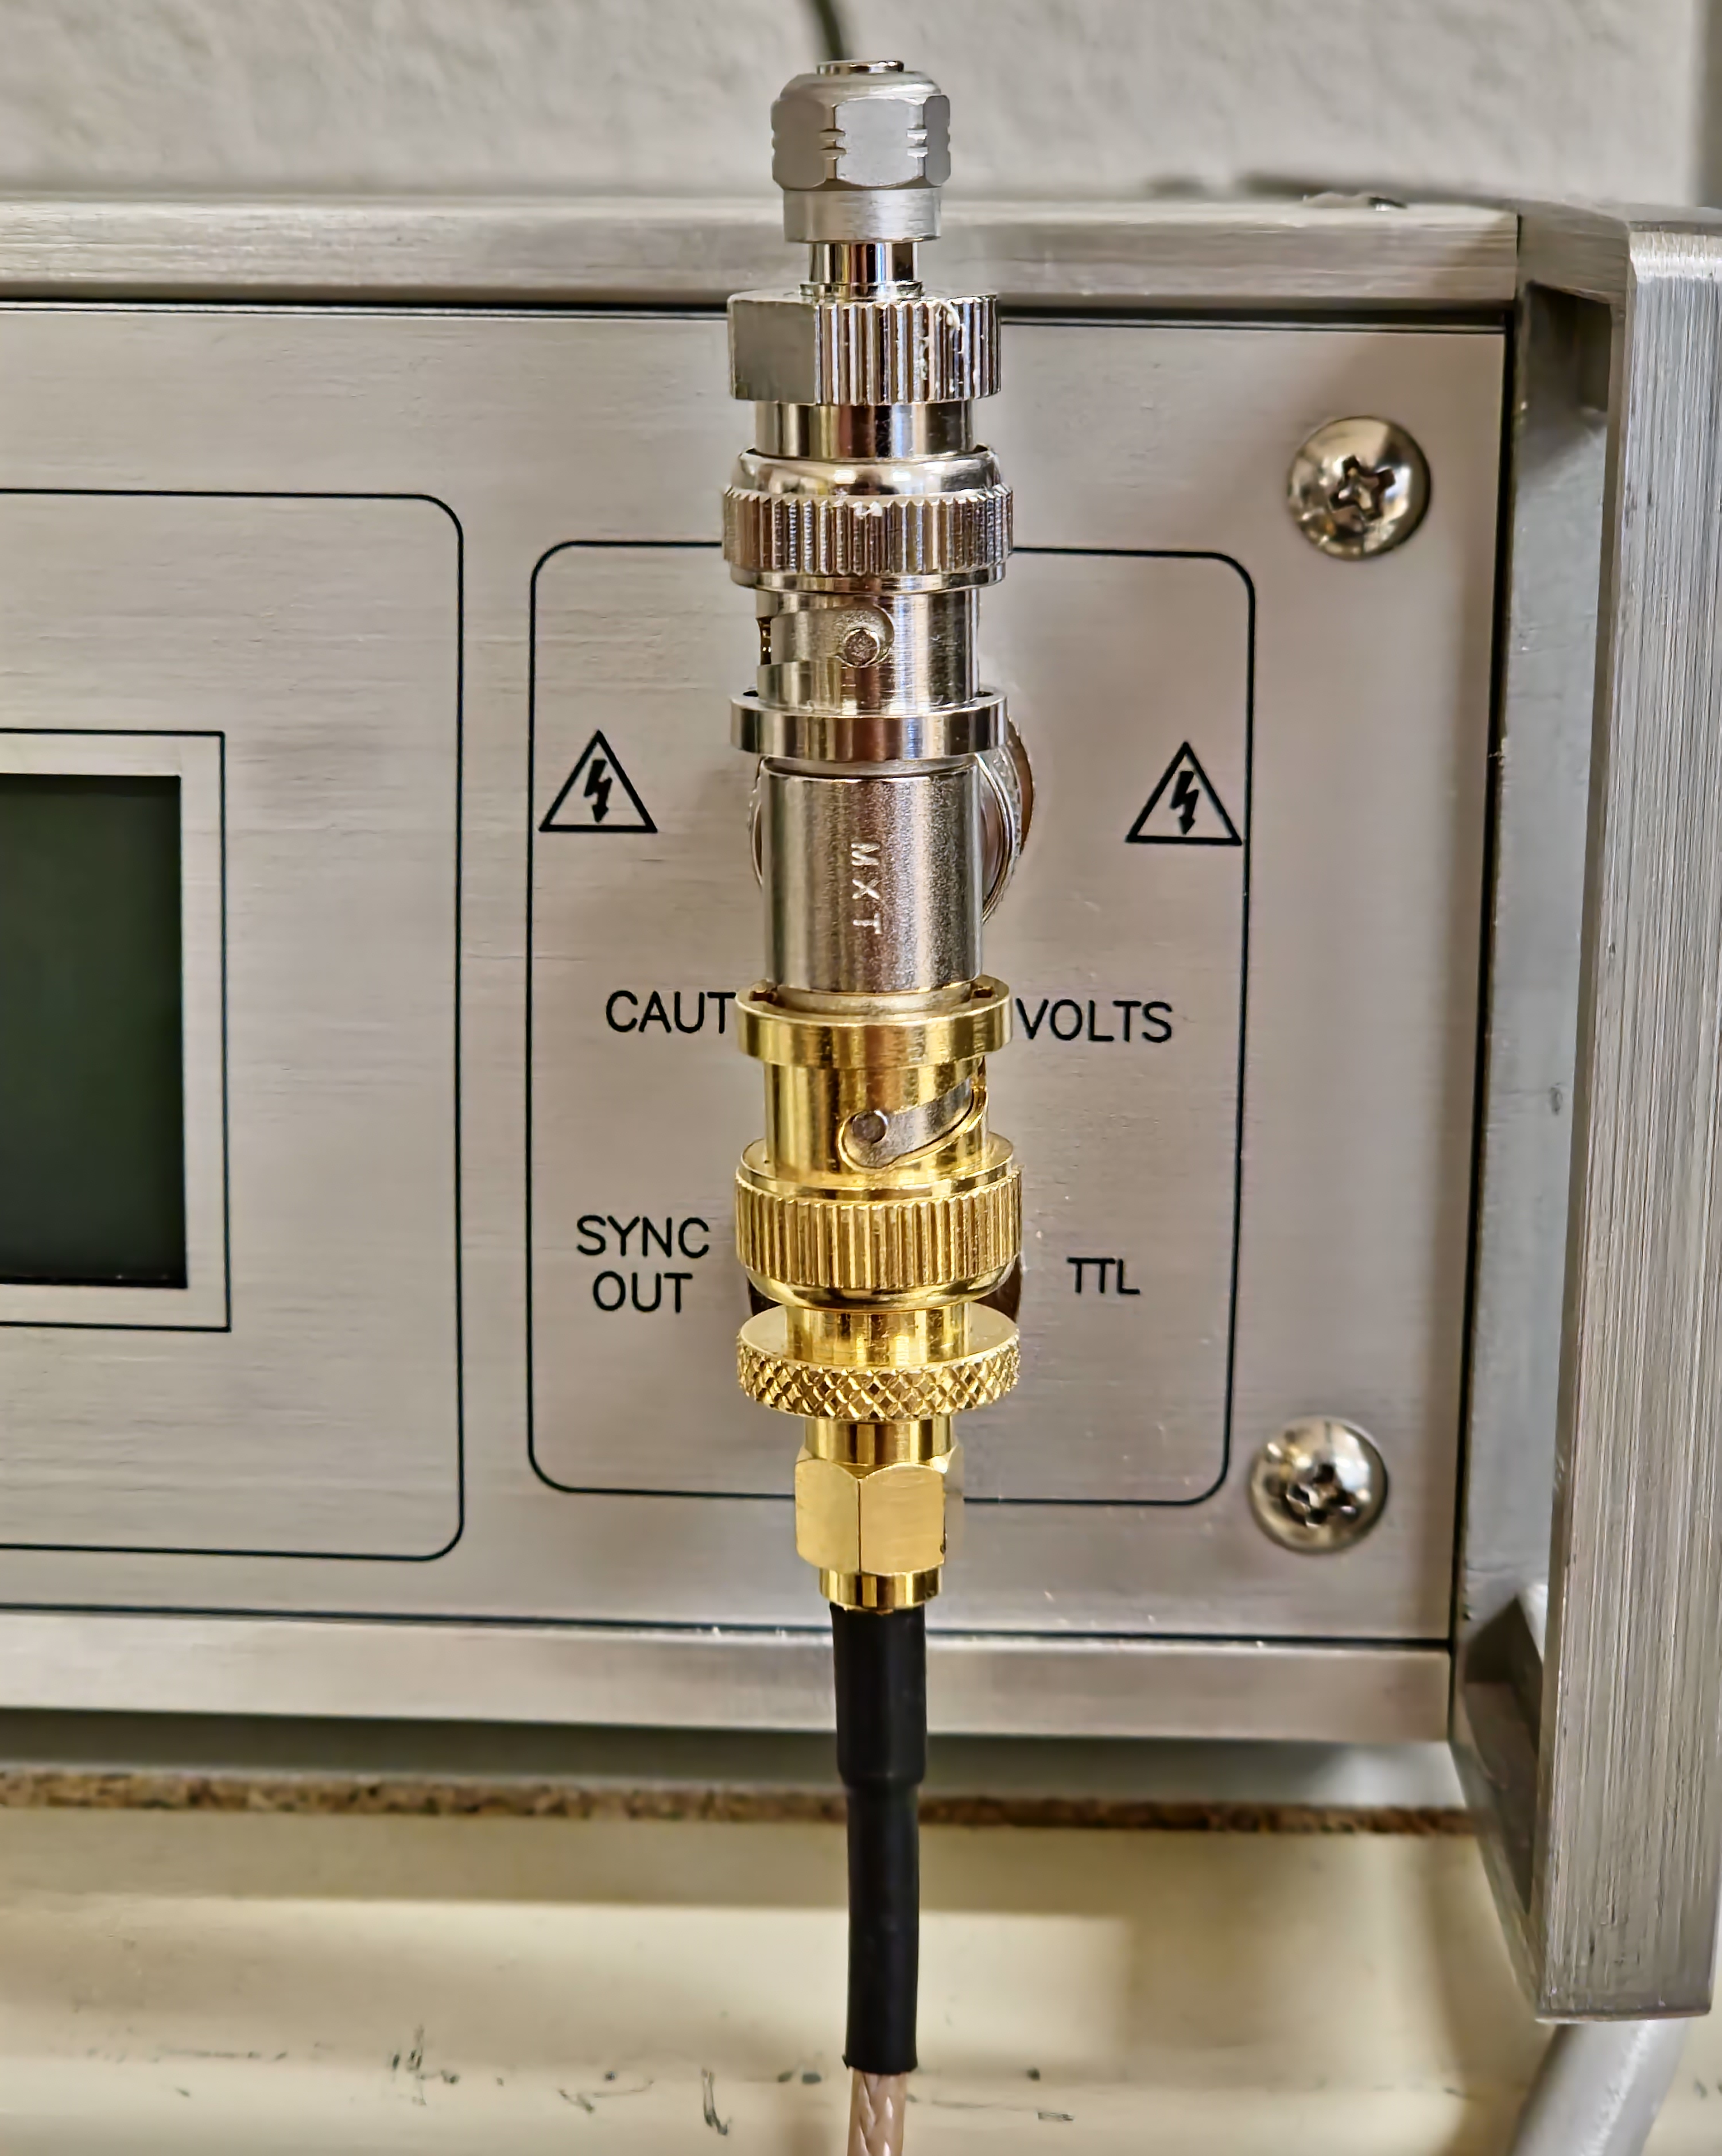
\includegraphics[width=0.60\textwidth, center]{2_goodPractices/figures/impMatchPicture.jpg}
        \caption{Actual implementation of the proposed impedance matching.}
        \label{fig:impMatchPhoto}
    \end{subfigure}
    \hfill
    \begin{subfigure}{0.48\textwidth}
        \centering
        \includegraphics[width=0.60\textwidth, center]{2_goodPractices/figures/sondeGndSource.jpg}
        \caption{Better alternative implementation of the impedance matching.}
        \label{fig:impMatchPhotoNew}
    \end{subfigure}
%    \hfill
    \caption{Actual pictures of a simple way to match the output impedance of the generator.}
    \label{fig:impMatch}
\end{figure}

    The impedance matching solution proposed and used during my experiments is shown in Fig. \ref{fig:impMatchPhoto}.
    However, it is far from being perfect.
    For instance, an ideal impedance matching implementation should be adaptive and dynamically change the impedance seen by the generator to perfectly match 50 \textOmega\xspace in every case.
    It would require a system with feedback, capable of measuring in real time the impedance presented by the IC target, in addition to the transmission line characteristics, to be able to dynamically adapt the compensation load impedance value.
    However, this is not the approach I have chosen.
    Indeed, the goal here is to minimize financial cost and platform modification, while allowing for better control over the platform parameters, whilst keeping a constant probe design.
    However, there is a trivial improvement which can be done, and is shown in Fig. \ref{fig:impMatchPhotoNew}.
    Instead of connecting the compensation load at the generator output, one can connect it at the transmission line output, also known as the probe input.
    Although it was not used during my experiments, it is a solution which can be considered.

    Another room for improvement would be to do a single and static measurement of the average IC backside impedance over its entire area, or over the targeted area (such as the cryptographic core, for instance).
    Then, thanks to this value, the compensation load impedance could be chosen to better match the required 50 \textOmega\xspace.

    Eventually, other shortcomings that neither of these solutions consider are the exact nature of the IC load.
    Indeed, the IC presents a complex impedance, which cannot be strictly approximated to a resistive load.
    Due to its internal structure, its impedance also has capacitive and inductive components.
    Therefore, considering them should lead to even better impedance matching.
%    Eventually, the solution I selected is fairly simple.
%    It consists in connecting a compensation load at the generator output, which is in a \fiftyOhms{50} SMA terminator.
%    The actual implementation is shown in Fig. \ref{fig:impMatchPhoto}.
%    It is far from ideal, as this solution does not consider the transmission line nor the IC effective load nor the capacitive and/or inductive nature of the IC in addition to its resistive nature.
    However, because the chosen solution requires little to no change to an existing platform and has proven to be good enough thanks to the previous models and the following results, I decided to stick to it.
%    A better approach would be to connect toe compensation load in parallel with the probe instead of the generator output.
%    I did not choose this option as it is probe dependent, while the generator option is universal and provides very good results.

    \subsection{Grounding installation bypass in practice \ddcu}
%    \textcolor{orange}{Add pictures of real GND bypass.}
    As I discussed previously, the grounding installation can drastically vary from one platform to another.
    Its effective impedance can be very high, such as in my platform, where equipment is grounded thanks to the platform earthing, with inter-equipment ground of around \fiftyOhms{150}.
    To alleviate the effects of such ground impedance, I simply decided to shunt the existing earthing with short low-resistance copper wires.
    To that end, I chose an arbitrary piece of equipment as the reference, and connected every other piece of equipment's local ground to the reference.
    It allowed reducing the effective platform ground impedance to a value close to \fiftyOhms{0}.

    \subsection{Practical analysis \ddcu}
    % !TeX root = ../0_Manuscript.tex

\begin{figure}[ht]
    \centering
    \includegraphics[width=1.0\textwidth, center]{2_goodPractices/figures/realPulsesComparisons.pdf}
    \caption{Actual \bbi platforms comparison: state-of-the-art (S1P and S1G) versus the proposed enhanced platform (S2P and S2G).}
    \label{fig:bbiRealXp}
\end{figure}
    Now that I presented how to practically set up the enhancements, let us analyze actual measurements on the platform.
    I will compare before and after results, allowing us to analyze each evaluation criterion.
    As it was done for the simulations, I will observe the voltage pulse and the IC ground current.

    Fig. \ref{fig:bbiRealXp} presents the various waveform results.
    The voltage pulse was measured at the IC backside during the injection, and the IC ground current was measured using a current probe thanks to the IC PCB ground interconnection.
    Therefore, the measured current is precisely the IC ground current, excluding any other equipment.
    The four waveforms displayed in Fig. \ref{fig:bbiRealXp} are code named using three characters for clarity.
    The first character is common to all waveforms, denoted “S” for “setup”.
    Then, the number indicates which platform is concerned, “1” being the default platform, “2” being the enhanced one.
    Eventually, the last letter indicates which waveform is observed, “P” being the voltage pulse, “G” being the IC ground current.
    Therefore, the default platform contains S1P and S1G waveforms, while the enhanced one contains S2P and S2G signals.
    Fig. \ref{fig:bbiRealXp} also displays the waveform characteristics for more clarity.
    The ideal voltage pulse applied has a maximum negative amplitude of 140 V, a pulse width of 20 ns, and 4 ns rise and fall times.

    S1P shows a clear undershoot of -108 \% under the set point.
    It is a clearly non-negligible value, which is far from desirable when performing fault injection, as usually, the voltage value has a great importance concerning efficiency and repeatability.
    In addition to this, the pulse width is 275 \% higher than its set point.
    It is an additional undesirable behavior, especially when one wants to inject precise disturbances into an IC under test.
    Then, fall time is four times higher than requested, and rise time is more than fifteen times higher.
    Put with the longer pulse width, it worsens the pulse accuracy.

    S1G brings to light the obvious ringing issue, also observable to a lesser extent on S1P, which leads to longer than expected disturbance inside the IC.
    Considering that the ringing is mainly caused by an impedance mismatch between the generator and the IC, it will drastically change from one location to another, further reducing repeatability.

    S2P, on the other hand, shows a better voltage amplitude, with a -31 \% undershoot.
    It is far from perfect, but given the approximate nature of the proposed impedance matching, it was to be expected.
    Concerning the pulse width, the set point value is perfectly respected, which is significant for precise disturbance duration.
    However, rise and fall times are now consistent, but still four times higher than requested.
    It can easily be explained by the fact that the transmission line, the probe, the IC and the power installation are not a purely resistive load.
    Therefore, any capacitive element in the chain will inevitably reduce the system response time, thus elongating rise and fall times, leading to a shorter pulse plateau.

    Concerning S2G, the approximate impedance matching shows a clear ringing reduction, with a steep current pulse, leading to a precise disturbance.
